% !TEX program = lualatex
% ECON 201, Worksheet 5: Profit and the Price of Cheerios. Compile with
% LuaLaTeX so the PDF is tagged (see syllabus/Econ201-Syllabus.tex for the
% same setup). Build from the course root:
%   latexmk -lualatex -cd worksheets/worksheet05.tex && latexmk -c -cd worksheets/worksheet05.tex
% Every number here is computed and printed by slides/figures/make_lecture5.py
% so the worksheet, the deck, and the debrief slide quote the same figures.
\DocumentMetadata{
  pdfstandard=UA-2,
  pdfversion=2.0,
  lang=en-US,
  tagging=on
}
\documentclass[11pt]{article}

\usepackage[letterpaper, margin=0.8in, top=0.6in, bottom=0.55in]{geometry}
\usepackage{fontspec}
\setmainfont{Fira Sans}
\usepackage{amsmath}
\usepackage{amssymb}
\usepackage{graphicx}
\usepackage{booktabs}
\usepackage{array}
% Questions are labelled by hand: under tagging=on, enumitem's enumerate
% did not step its counter, so every item printed the same label.
\newcounter{q}
\newcommand{\Q}[1]{\stepcounter{q}\par\needspace{5\baselineskip}\vspace{3pt}\noindent\hangindent=1.7em\hangafter=1
  \makebox[1.7em][l]{(\alph{q})}#1\par}
\usepackage{xcolor}
\usepackage{needspace}
\definecolor{accent}{HTML}{BF5700}
\usepackage{titlesec}
\titleformat{\section}{\large\bfseries\color{accent}}{}{0pt}{}
\titlespacing*{\section}{0pt}{6pt}{2pt}
\usepackage{hyperref}
\hypersetup{pdftitle={ECON 201 Worksheet: Profit and the Price of Cheerios}, pdfauthor={Div Bhagia}, hidelinks}
\pagestyle{empty}
\setlength{\parindent}{0pt}
\setlength{\parskip}{3pt}

% Ruled answer space: n lines. Plain TeX loop; pgffor's \foreach breaks the
% enumerate counter when used inside an item.
\newcount\answerlinecount
\newcommand{\answerlines}[1]{%
  \par\vspace{1pt}\answerlinecount=#1
  \loop\ifnum\answerlinecount>0
    \rule{\linewidth}{0.3pt}\par\vspace{5pt}%
    \advance\answerlinecount by -1
  \repeat
  \vspace{-5pt}}

\begin{document}

{\LARGE\bfseries\color{accent} Worksheet: Profit and the Price of Cheerios}\hfill{\large ECON 201}

\vspace{2pt}
Work with a neighbor. Write your answers in the spaces.

Three definitions you will use throughout this module. \emph{Total revenue}
is the number of units sold times the price per unit: $R = P \times Q$.
\emph{Total cost}, written $C(Q)$, is the cost of producing $Q$ units.
\emph{Profit} is total revenue minus total cost:
\[
\text{Profit} = \underbrace{P \times Q}_{\text{revenue, } R} - \underbrace{C(Q)}_{\text{total cost}}
\]

\needspace{7\baselineskip}\section{1. Do higher prices always mean higher profits?}\setcounter{q}{0}

A firm's profit is $P \times Q - C(Q)$. To maximize profit, why not just
charge a really high price? Jot down your thoughts, then compare answers
with a neighbor.
\answerlines{4}

\needspace{10\baselineskip}\section{2. Pricing Apple Cinnamon Cheerios}\setcounter{q}{0}

You are the manager at General Mills who sets the price of Apple Cinnamon
Cheerios. Producing the cereal costs \$2.00 per pound, so producing $Q$
pounds costs $C(Q) = 2Q$. Market research, based on the demand curve the
economist Jerry Hausman estimated for this cereal, tells you how many pounds
a typical city buys each week at each price:

% A ruled grid rather than a booktabs table: students write in the cells,
% so every cell gets visible borders and the blank rows get extra height.
\begin{center}
\renewcommand{\arraystretch}{1.5}
\newcolumntype{C}{>{\centering\arraybackslash}p{2.0cm}}
\begin{tabular}{|>{\raggedright\arraybackslash}p{3.6cm}|C|C|C|C|C|}
\hline
Price per pound, $P$ & \$3.00 & \$3.50 & \$4.00 & \$4.50 & \$5.00 \\
\hline
Pounds sold per week, $Q$ & 25,000 & 21,000 & 17,000 & 13,000 & 9,000 \\
\hline
Total revenue, $R$ & \rule{0pt}{2.4em} & & & & \\
\hline
Total cost, $C$ & \rule{0pt}{2.4em} & & & & \\
\hline
Profit & \rule{0pt}{2.4em} & & & & \\
\hline
\end{tabular}
\end{center}

\Q{Fill in total revenue, total cost, and profit at each price.}

\Q{Which price would you set, and what is the weekly profit there?}
\answerlines{2}

\Q{Plot the five columns of your table on the four grids below, one point
per column on each grid, and connect the points: the demand curve ($P$
against $Q$), total revenue $R$, total cost $C$, and profit.}

\begin{center}
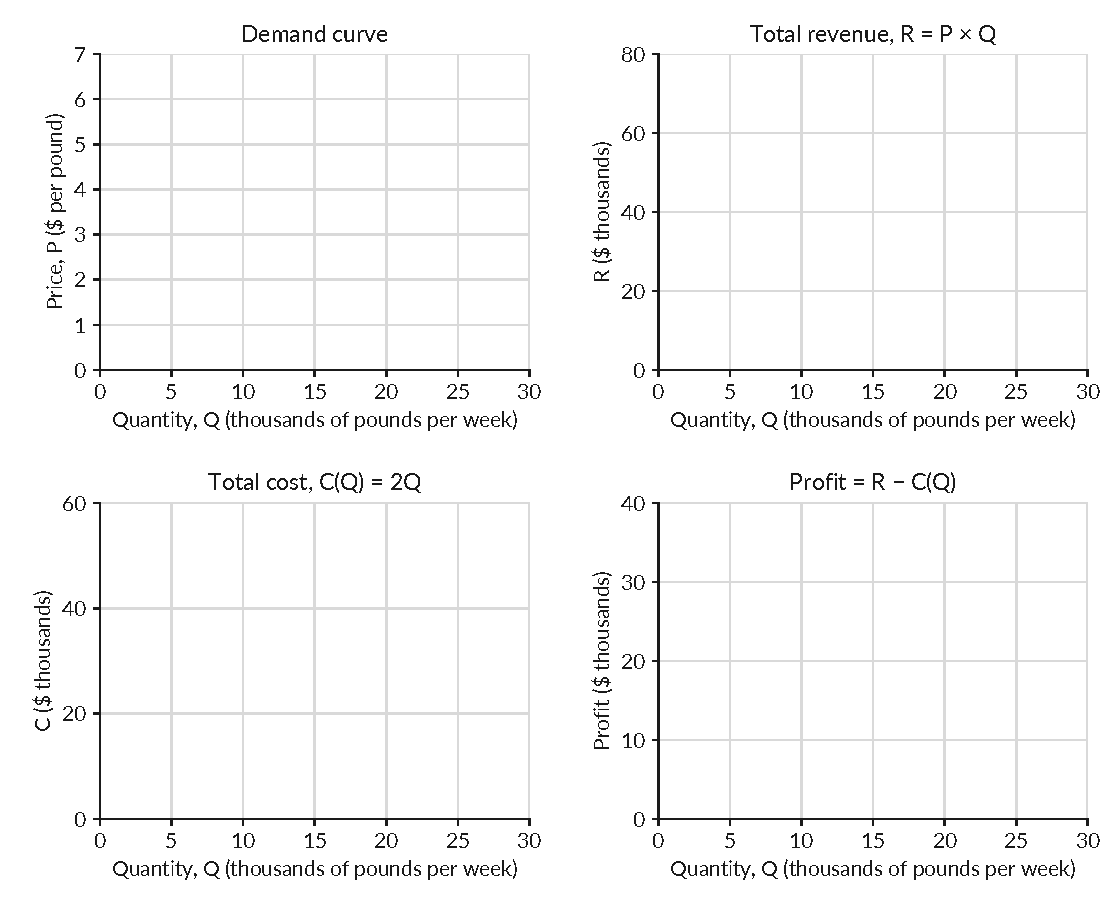
\includegraphics[width=\textwidth, alt={Four empty plotting grids with
light gridlines, each with quantity Q in thousands of pounds per week from
0 to 30 on the horizontal axis. Top left: demand curve, price P from 0 to 7
dollars per pound. Top right: total revenue R from 0 to 80 thousand
dollars. Bottom left: total cost C from 0 to 60 thousand dollars. Bottom
right: profit from 0 to 40 thousand dollars.}]{figures/cheerios-grid.pdf}
\end{center}

\Q{Total revenue is highest at \$3.00, yet that is not the most profitable
price. Explain why in a sentence or two.}
\answerlines{3}

\Q{Why does profit fall when you raise the price from \$4.00 to \$5.00, even
though you earn a bigger margin on every pound?}
\answerlines{3}

\end{document}
